\documentclass[12pt]{report}
\usepackage[utf8]{inputenc}
\usepackage[russian]{babel}
\linespread{1.5}
%\usepackage[14pt]{extsizes}
\usepackage{listings}
\usepackage{float}
\usepackage{graphicx}
\usepackage[left=2cm,right=2cm,
    top=2cm,bottom=2cm,bindingoffset=0cm]{geometry}
\usepackage{amsmath,amsfonts,amssymb,amsthm,mathtools} 

% Для листинга кода:
\lstset{ %
language=swift,                
basicstyle=\small\sffamily, % размер и начертание шрифта для подсветки кода
numbers=left,               % где поставить нумерацию строк (слева\справа)
numberstyle=\tiny,           % размер шрифта для номеров строк
stepnumber=1,                   % размер шага между двумя номерами строк
numbersep=5pt,                % как далеко отстоят номера строк от подсвечиваемого кода
showspaces=false,            % показывать или нет пробелы специальными отступами
showstringspaces=false,      % показывать или нет пробелы в строках
showtabs=false,             % показывать или нет табуляцию в строках
frame=single,              % рисовать рамку вокруг кода
tabsize=2,                 % размер табуляции по умолчанию равен 2 пробелам
captionpos=t,              % позиция заголовка вверху [t] или внизу [b] 
breaklines=true,           % автоматически переносить строки (да\нет)
breakatwhitespace=false, % переносить строки только если есть пробел
escapeinside={\#*}{*)}   % если нужно добавить комментарии в коде
}

% Для измененных титулов глав:
%\usepackage{titlesec, blindtext, color} % подключаем нужные пакеты
%\definecolor{gray75}{gray}{0.75} % определяем цвет
%\newcommand{\hsp}{\hspace{20pt}} % длина линии в 20pt
% titleformat определяет стиль
%\titleformat{\chapter}[hang]{\Huge\bfseries}{\thechapter\hsp\textcolor{gray75}{|}\hsp}{0pt}{\Huge\bfseries}

\usepackage{titlesec}
\titleformat{\chapter}[block]
  {\normalfont\huge\bfseries}{\thechapter.}{1em}{\Huge}
\titlespacing*{\chapter}{0pt}{-19pt}{0pt}


% plot
\usepackage{pgfplots}
\usepackage{filecontents}
\usetikzlibrary{datavisualization}
\usetikzlibrary{datavisualization.formats.functions}
\newenvironment{comment}{}{}

\begin{document}


%\def\chaptername{} % убирает "Глава"
\begin{titlepage}

	\fontsize{12pt}{12pt}\selectfont
	\noindent \begin{minipage}{0.15\textwidth}
		
\includegraphics[width=\linewidth]{b_logo.jpg}
	\end{minipage}
	\noindent\begin{minipage}{0.9\textwidth}\centering
		\textbf{Министерство науки и высшего образования Российской Федерации}\\
		\textbf{Федеральное государственное бюджетное образовательное учреждение высшего образования}\\
		\textbf{«Московский государственный технический университет имени Н.Э.~Баумана}\\
		\textbf{(национальный исследовательский университет)»}\\
		\textbf{(МГТУ им. Н.Э.~Баумана)}
	\end{minipage}
	
	\noindent\rule{18cm}{3pt}
	\newline\newline
	\noindent ФАКУЛЬТЕТ $\underline{\textbf{«Информатика и системы управления»}}$ \newline\newline
	\noindent КАФЕДРА $\underline{\textbf{«Программное обеспечение ЭВМ и информационные технологии»}}$\newline\newline\newline\newline
	
	\begin{center}
		\Large\textbf{Отчет по лабораторной работе №2 по курсу <<Анализ алгоритмов>>}
	\end{center}
	\newline\newline 
	\newline
	
	\noindent\textbf{Тема} $\underline{\textbf{Алгоритмы умножения матриц~~~~~~~~~~~~~~~~~~~~~~~~~~~}}$\newline\newline
	\noindent\textbf{Студент} $\underline{\textbf{Челядинов И.Д.~~~~~~~~~~~~~~~~~~~~~~~~~~~~~~~~~}}$\newline\newline
	\noindent\textbf{Группа} $\underline{\textbf{ИУ7-53Б~~~~~~~~~~~~~~~~~~~~~~~~~~~~~~~~~~~~~~~~~~~~}}$\newline\newline
	\noindent\textbf{Оценка (баллы)} $\underline{\textbf{~~~~~~~~~~~~~~~~~~~~~~~~~~~~~~~~~~~~~~~~~~}}$\newline\newline
	\noindent\textbf{Преподаватели} $\underline{\textbf{Волкова Л.Л., Строганов Ю.В.}}$\newline
	
	\begin{center}
		\vfill
		Москва~---~\the\year
		~г.
	\end{center}
 \restoregeometry
\end{titlepage}


\tableofcontents
\newpage
\chapter*{Введение}
\addcontentsline{toc}{chapter}{Введение}
Цель работы: изучение алгоритмов умножения матриц. В данной лабораторной работе рассматривается стандартный алгоритм умножения матриц, алгоритм Винограда и модифицированный алгоритм Винограда.  Также требуется изучить рассчет сложности алгоритмов, получить навыки в улучшении алгоритмов.

Матрицей A размера $[m*n]$ называется таблица элементов, расположение которых определяется при помощи порядкового номера столбца и строки. Важнейшие характеристики матрицы - число строк и число столбцов. Сами числа называют элементами матрицы и характеризуют их положением в матрицы, задавая номер строки и столбца и записывая их в виде двойного индекса, причем вначале записывают номер строки, затем номер столбца.
Пусть есть два конечных множества.
\begin{itemize}
	\item номера строк: M = 1, 2, ..., n;
	\item Номера столбцов N = 1, 2, ..., m;
\end{itemize}
где m и n - натуральные числа.
Тогда матрица A представлена на рисунке 1:
\begin{figure}[H]
    \centering
    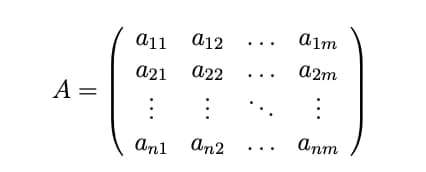
\includegraphics[width=0.70\linewidth]{7.jpg}
    \caption{Сравнение времени работы при разном размере матрицы}
    \label{fig:mpr}
\end{figure}
\newline
Простейшими действиями над матрицами являются следующие операции.

\begin{enumerate}
	\item Умножение матрицы на число. Для этого необходимо умножить каждый элемент матрицы на данное число.
	\item Сложение матриц. Складывать можно только матрицы одинакового размера, то есть, имеющие  одинаковое число строк и одинаковое число столбцов. При сложении матриц соответствующие их элементы складываются;
	\item Транспонирование матрицы. При транспонировании у матрицы строки становятся столбцами и наоборот.
\end{enumerate}
В ходе лабораторной работы предстоит:
\begin{itemize}
	\item изучить алгоритмы умножения матриц: стандартный алгоритм и алгоритм Винограда;
	\item оптимизировать алгоритм Винограда;
	\item дать теоретическую оценку базового алгоритма умножения матриц, алгоритма Винограда и улучшенного алгоритма Винограда;
	\item реализовать три алгоритма умножения матриц на одном из языков программирования;
	\item сравнить алгоритмы умножения матриц.
\end{itemize}

\chapter{Аналитическая часть}
Произведение матриц AB состоит из всех возможных комбинаций скалярных произведений вектор-строк матрицы А и вектор-столбцов матрицы В.
Операция умножения двух матриц выполнима только в том случае, если число столбцов в первой матрицы равно числу строк во второй.


\section{Алгоритм Винограда}
Подход Алгоритма Винограда является иллюстрацией общей методологии, начатой в 1979-х годах на основе
билинейных и трилинейных форм, благодаря которым большинство усовершенствований для умножения матриц были получены. \cite{vinograd}.

Рассмотрим два вектора $V = (v1, v2, v3, v4)$ и $W = (w1, w2, w3, w4)$.  

 Их скалярное произведение равно (\ref{formula}) 

\begin{equation} \label{formula}
V \cdot W=v_1 \cdot w_1 + v_2 \cdot w_2 + v_3 \cdot w_3 + v_4 \cdot w_4
\end{equation}

Равенство (\ref{formula}) можно переписать в виде (\ref{formula2}) 
\begin{equation} \label{formula2}
V \cdot W=(v_1 + w_2) \cdot (v_2 + w_1) + (v_3 + w_4) \cdot (v_4 + w_3) - v_1 \cdot v_2 - v_3 \cdot v_4 - w_1 \cdot w_2 - w_3 \cdot w_4
\end{equation}

Менее очевидно, что выражение в правой части последнего равенства допускает предварительную обработку: его части можно вычислить заранее и запомнить для каждой строки первой матрицы и для каждого столбца второй. 
Это означает, что над предварительно обработанными элементами нам придется выполнять лишь первые два умножения и последующие пять сложений, а также дополнительно два сложения. 

\section{Вывод}
Были рассмотрены алгоритмы классического умножения матриц и алгоритм Винограда, основное отличие которых — наличие предварительной обработки, а также количество операций умножения.



\chapter{Конструкторская часть}
\textbf{Требования к вводу:}
На вход подаются две матрицы
\newline
\textbf{Требования к программе:}
\begin{itemize}
\item корректное умножение двух матриц;
\item при матрицах неправильных размеров программа не должна аварийно завершаться.
\end{itemize}

\section{Схемы алгоритмов}
В данной части будут рассмотрены схемы алгоритмов.

На рисунке 2.1 представлен алгоритм классического умножения матриц.
\begin{figure}[H]
    \centering
    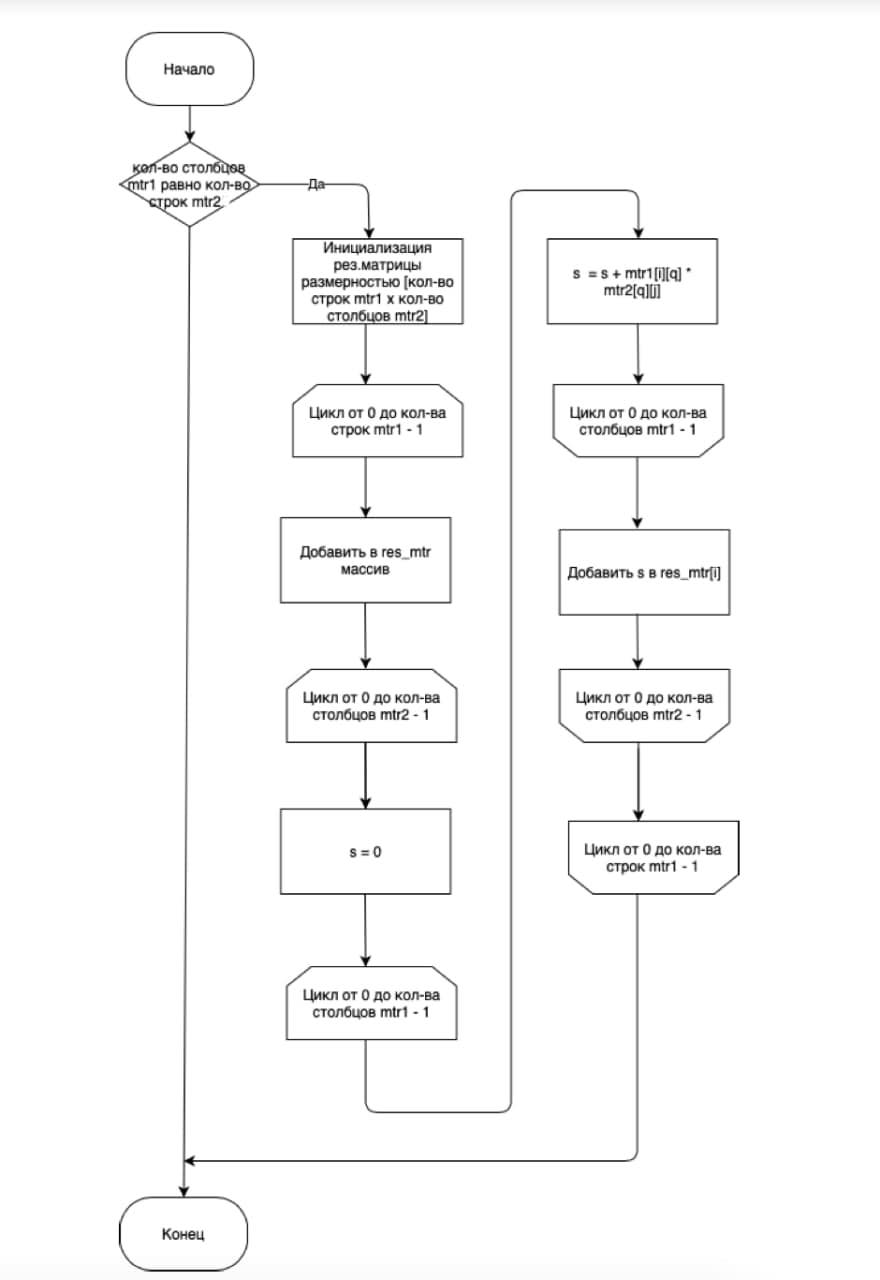
\includegraphics[width=0.70\linewidth]{1.jpg}
    \caption{Схема классического умножения матриц}
    \label{fig:mpr}
\end{figure}

На рисунках 2.2 - 2.3 представлен алгоритм умножения матриц по Винограду.
\begin{figure}[H]
    \centering
    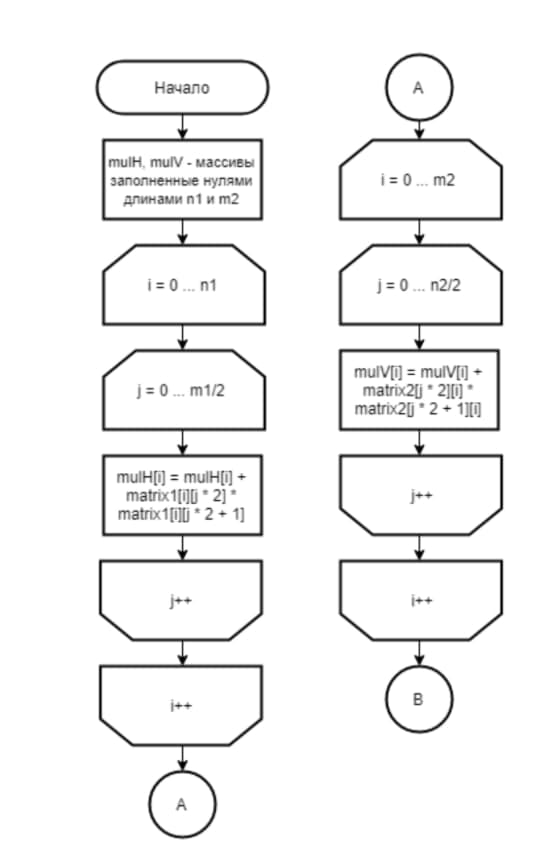
\includegraphics[width=0.70\linewidth]{2.jpg}
    \caption{}
    \label{fig:mpr}
\end{figure}

\begin{figure}[H]
    \centering
    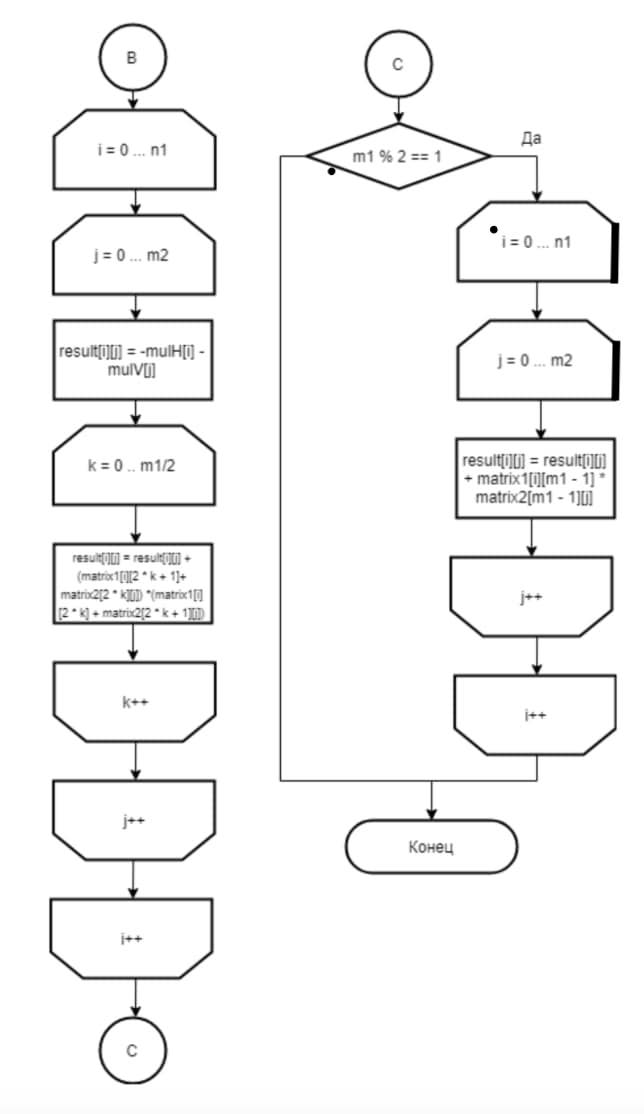
\includegraphics[width=0.70\linewidth]{3.jpg}
    \caption{Схема алгоритма Винограда}
    \label{fig:mpr}
\end{figure}

На рисунках 2.4 - 2.5 представлен оптимизированный алгоритм умножения матриц по Винограду.
\begin{figure}[H]
    \centering
    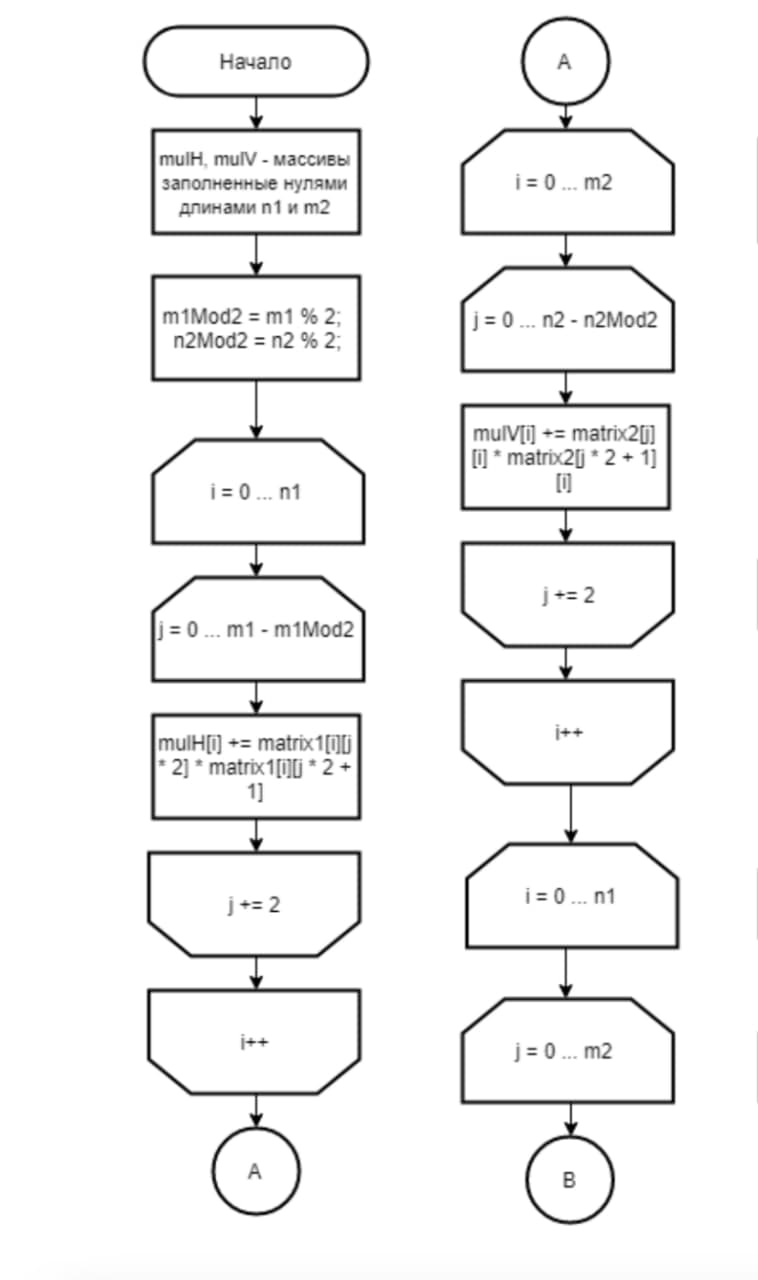
\includegraphics[width=0.70\linewidth]{4.jpg}
    \caption{ }
    \label{fig:mpr}
\end{figure}

\begin{figure}[H]
    \centering
    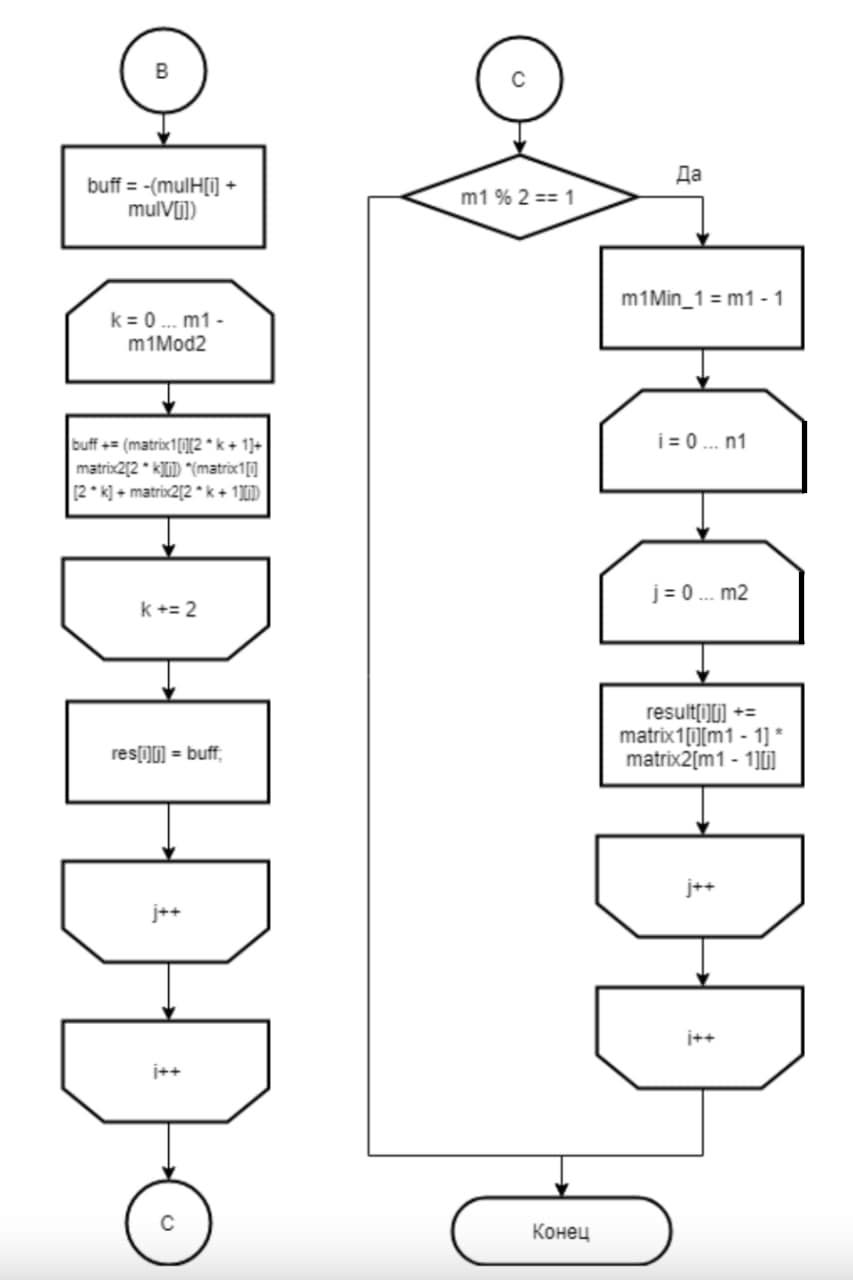
\includegraphics[width=0.70\linewidth]{5.jpg}
    \caption{Схема оптимизированного алгоритма Винограда}
    \label{fig:mpr}
\end{figure}
\newline

\chapter{Технологическая часть}
\section{Выбор ЯП}
В качестве языка программирования был выбран Golang, Goland была выбрана в качестве среды разработки. \cite{Golang} \cite{Goland}
Такой выбор средств выполнения лабораторной работы был связан с наличием в языке Golang системы тестирования "Benchmark", которая позволяет быстро и качественно произвести тестирование программы и замерить время с высокой точностью.


\section{Сведения о модулях программы}
Программа состоит из:
\begin{itemize}
	\item main.go - главный файл программы, в котором располагается точка входа в программу и функции перемножения матриц.
	\item algh_test.go - файл с benchmark тестами.
\end{itemize}


\section{Листинг кода алгоритмов}

В листинге 3.1 представлена функция инициализации матрицы.
\begin{lstlisting}[label=CodeStand,caption= Инициализация матрицы]
func createMatrix(row, col int) [][]int {
	matrix := make([][]int, row)
	for i := range matrix {
		matrix[i] = make([]int, col)
	}
	return matrix
}

\end{lstlisting}

В листинге 3.2 представлена функция стандартного умножения матриц.
\newline
\begin{lstlisting}[label=CodeStand,caption= Стандартный алгоритм умножения матриц]
func StandartMult(m1, m2 [][]int) [][]int {
	if (len(m1) == 0 || len(m2) == 0) || (len(m1[0]) != len(m2)) {
		return nil
	}
	res := createMatrix(len(m1), len(m2[0]))
	for i := 0; i < len(m1); i++ {
		for j := 0; j < len(m2[0]); j++ {
			for k := 0; k < len(m2); k++ {
				res[i][j] += m1[i][k] * m2[k][j]
			}
		}
	}
	return res
}
\end{lstlisting}

В листинге 3.3 представлена функция умножения матриц по Винограду.
\begin{lstlisting}[label=some-code,caption=Алгоритм Винограда]
func VinogradMult(m1, m2 [][]int) [][]int {
	if (len(m1) == 0 || len(m2) == 0) || (len(m1[0]) != len(m2)) {
		return nil
	}
	res := createMatrix(len(m1), len(m2[0]))
	rowF := make([]int, len(m1))
	colF := make([]int, len(m2[0]))

	for i := 0; i < len(m1); i++ {
		for j := 0; j < len(m1[0])/2; j++ {
			rowF[i] += m1[i][j*2] * m1[i][j*2+1]
		}
	}

	for i := 0; i < len(m2[0]); i++ {
		for j := 0; j < len(m2)/2; j++ {
			colF[i] += m2[j*2][i] * m2[j*2+1][i]
		}
	}

	for i := 0; i < len(m1); i++ {
		for j := 0; j < len(m2[0]); j++ {
			res[i][j] = -rowF[i] - colF[j]
			for k := 0; k < len(m1[0])/2; k++ {
				res[i][j] += (m1[i][2*k+1] + m2[2*k][j]) * (m1[i][2*k] + m2[2*k+1][j])
			}
		}
	}

	if len(m1[0])%2 == 1 {
		for i := 0; i < len(m1); i++ {
			for j := 0; j < len(m2[0]); j++ {
				res[i][j] += m1[i][len(m1[0])-1] * m2[len(m1[0])-1][j]
			}
		}
	}
	return res
}
\end{lstlisting}

В листинге 3.4 представлен код функции оптимизированного умножения матриц по Винограду.
\begin{lstlisting}[label=some-code,caption=Оптимизированный алгоритм Винограда]
func VinOptimMult(matrix1 [][]int, matrix2 [][]int) [][]int {
	var n1 int = len(matrix1)
	var n2 int = len(matrix2)

	if n1 == 0 || n2 == 0 {
		return nil
	}

	var m1 int = len(matrix1[0])
	var m2 int = len(matrix2[0])

	if m1 != n2 {
		return nil
	}

	mulH := make([]int, n1)
	mulV := make([]int, m2)
	result := createMatrix(n1, m2)

	var m1Mod2 int = m1 % 2
	var n2Mod2 int = n2 % 2

	for i := 0; i < n1; i++ {
		for j := 0; j < m1-m1Mod2; j += 2 {
			mulH[i] += matrix1[i][j] * matrix1[i][j+1]
		}
	}

	for i := 0; i < m2; i++ {
		for j := 0; j < n2-n2Mod2; j += 2 {
			mulV[i] += matrix2[j][i] * matrix2[j+1][i]
		}
	}

	var buff int
	for i := 0; i < n1; i++ {
		for j := 0; j < m2; j++ {
			buff = -mulH[i] - mulV[j]
			for k := 0; k < m1-m1Mod2; k += 2 {
				buff += (matrix1[i][k+1] + matrix2[k][j]) * (matrix1[i][k] + matrix2[k+1][j])
			}
			result[i][j] = buff
		}
	}

	if m1Mod2 == 1 {
		var m1Min1 int = m1 - 1
		for i := 0; i < n1; i++ {
			for j := 0; j < m2; j++ {
				result[i][j] += matrix1[i][m1Min1] * matrix2[m1Min1][j]
			}
		}
	}

	return result
}
\end{lstlisting}

\section{Вывод}
В данном разделе мы рассмотрели листинг программы и структуру программы.

\chapter{Исследовательская часть}

\section{Сравнительный анализ на основе замеров времени работы алгоритмов}

Был проведен замер времени работы каждого из алгоритмов. Замер производился на ноутбуке Macbook pro 13 на базе процессоре Intel core i5, который обладает  1.4 GHz тактовой частоты, а также 8 гигабайтами оперативной памяти.\cite{computer}\cite{intel} Для произведения замера времени использовалась система тестирования Benchmark языка Golang.
Данная система тестирования позволяет измерить скорость работы алгоритма с минимальной погрешностью. \newline
На рисунке 4.1 представлена сравнительная характеристика времени работы программы при четных размерах матрицы.
\begin{figure}[H]
    \centering
    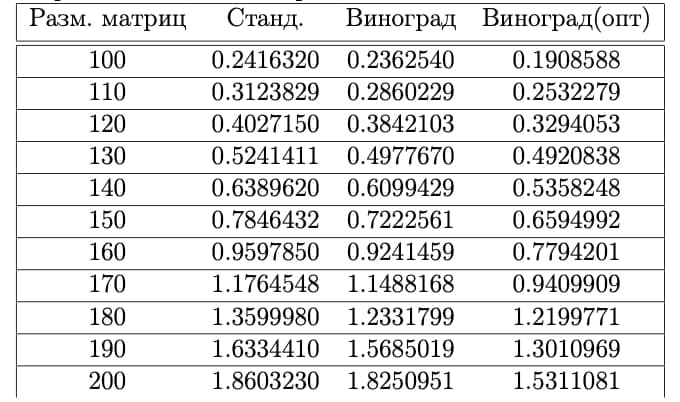
\includegraphics[width=0.70\linewidth]{8.jpg}
    \caption{Сравнительная характеристика времени работы программы при четных размерах матрицы}
    \label{fig:mpr}
\end{figure}
\newline
\newpage


Первый эксперимент производится для лучшего случая на квадратных матрицах размером от 100 x 100 до 1000 x 1000 c шагом 100. 
Сравним результаты для разных алгоритмов:

На рисунке 4.2 представлено сравнение времени работы при разном размере матрицы.
\begin{figure}[H]
    \centering
    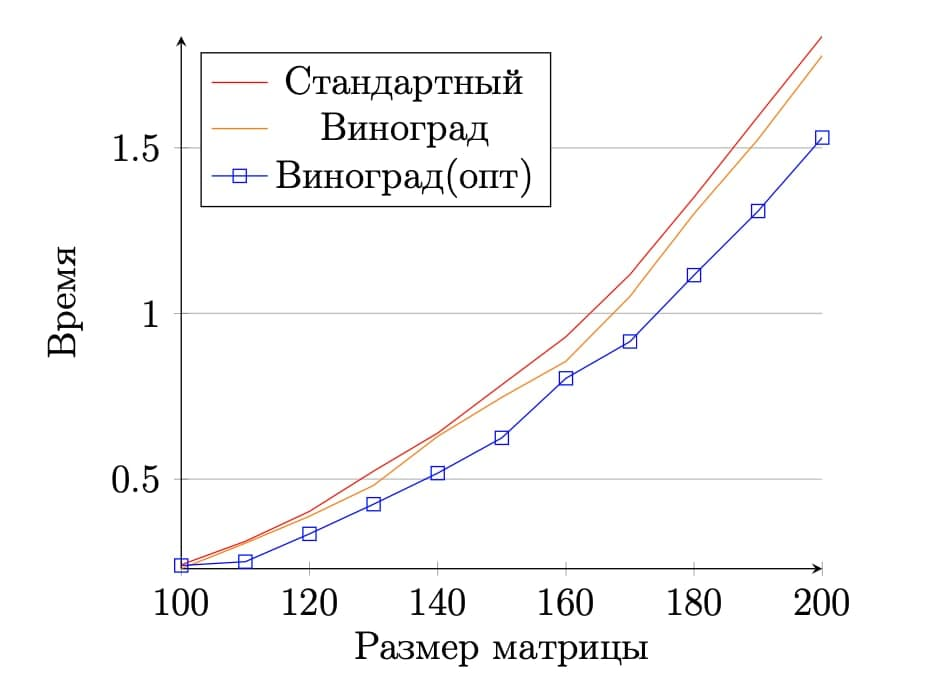
\includegraphics[width=0.70\linewidth]{6.jpg}
    \caption{Сравнение времени работы при разном размере матрицы}
    \label{fig:mpr}
\end{figure}
\newline
\newpage



\section{Вывод}
По результатам тестирования, а также оценке времени работы, данные алгоритмы реализованы верно. Самым медлен
По результатам тестирования все рассматриваемые алгоритмы реализованы правильно. Самым медленным алгоритмом оказался алгоритм классического умножения матриц, а самым быстрым — оптимизированный алгоритм Винограда.

\newpage
\addcontentsline{toc}{chapter}{Литература}
\bibliographystyle{utf8gost705u}  % стилевой файл для оформления по ГОСТу
\nocite{*}
\bibliography{51-biblio} 
\end{document}
